\documentclass[11pt]{article}
\usepackage[top=1in, bottom=1in, left=1.25in, right=1.25in]{geometry}
\usepackage[BoldFont,SlantFont,CJKsetspaces,CJKchecksingle]{xeCJK}
\usepackage{framed}
\usepackage{amsmath}
\usepackage{listings}
\setCJKmainfont[BoldFont=SimHei]{SimSun}
\setCJKmonofont{SimSun}
\usepackage{graphicx}
\usepackage{color}
\definecolor{mygreen}{rgb}{0,0.6,0}
\definecolor{mygray}{rgb}{0.5,0.5,0.5}
\definecolor{mymauve}{rgb}{0.58,0,0.82}
\lstset{ %
  backgroundcolor=\color{white},
  basicstyle=\ttfamily,
  breakatwhitespace=false,
  breaklines=true,
  captionpos=t,
  commentstyle=\color{mygreen},
  columns=flexible,
  deletekeywords={...},
  escapeinside={\%*}{*)},
  extendedchars=true,
  frame=single,
  keepspaces=true,
  keywordstyle=\color{blue},
  language=C,
  morekeywords={*,...},
  numbers=none,
  rulecolor=\color{black},
  showspaces=false,
  showstringspaces=false,
  showtabs=false,
  stepnumber=1,
  stringstyle=\color{mymauve},
  tabsize=2,
  title=\lstname
}
\newenvironment{packed_enum}{
\begin{enumerate}
  \setlength{\itemsep}{1pt}
  \setlength{\parskip}{0pt}
  \setlength{\parsep}{0pt}
}{\end{enumerate}}
\parindent 2em

\begin{document}
\title{\textbf{\huge{实验报告 Lab2}}\\
10300240039 章超}
\maketitle
\section{Physical Page Management}
\begin{framed}
\noindent\textbf{Exercise 1}In the file \lstinline|kern/pmap.c|, you must implement code for the following functions (probably in the order given).

\begin{lstlisting}[frame=none,aboveskip=-1.5em]
boot_alloc()
mem_init() (only up to the call to check_page_free_list(1))
page_init()
page_alloc()
page_free()
\end{lstlisting}

\lstinline|check_page_free_list()| and \lstinline|check_page_alloc()| test your physical page allocator. You should boot JOS and see whether \lstinline|check_page_alloc()| reports success. Fix your code so that it passes. You may find it helpful to add your own \lstinline|assert()|s to verify that your assumptions are correct.
\end{framed}
这一部分的实验要求是完成物理页面分配的相关函数。从Lab1中,我们已经知道JOS启动时先载入Boot loader, 然后Boot loader载入Kernel。Kernel初始化时调用\lstinline|i386_init()|,并且\lstinline|i386_init()|在控制台相关函数初始化后调用\lstinline|mem_init()|,也就是Lab2实验的入口。

在调用\lstinline|i386_init()|之前,JOS的物理内存占用情况如下:

\begin{tabular}{rll}
0x100000(1MB) & -end: & Kernel Code\\
0xA0000(640KB) & -0x100000(1MB): & Bios data, Video ram\\
0x10000 & -?: & ELF Header\\
0x7C00 & -?: & Boot sector code\\
0x0 & -0x1000: & Real Mode IDT
\end{tabular}

\subsection{\lstinline|boot_alloc()|}

首先看到\lstinline|mem_init()|调用了\lstinline|boot_alloc()|,
\begin{lstlisting}[title=kern/pmap.c]
kern_pgdir = (pde_t *) boot_alloc(PGSIZE);
memset(kern_pgdir, 0, PGSIZE);
\end{lstlisting}

注释中提到了这一部分创建了页的目录,我们找到页目录的定义如下:

\begin{lstlisting}[title=inc/memlayout.h]
struct PageInfo {
	struct PageInfo *pp_link;
	uint16_t pp_ref;
};
\end{lstlisting}

从这个定义可以看到,每个页目录包含两个值,一个是在Free list链表中的下一个页的地址,另外一个是该页引用次数。Free list是一个空闲页的链表,每次申请页面时,Free List头指针向后移,并将原先所指的页分配;每次释放页面时,将页面在头部插入Free list。这个页的引用次数则用于标明一个页面是否可以被释放,如果在\lstinline|page_free()|后,这个页面引用为0,那么就可以释放。

每个物理页目录可以与虚拟地址相互转换,也可以与物理地址相互转换,具体的代码已经实现了,可以参考\lstinline|pmap.h|中的宏。如\lstinline|page2pa(struct PageInfo *pp)|返回物理页目录对应的物理地址,\lstinline|pa2page(physaddr_t pa)|返回物理地址对应的页,\lstinline|page2kva(struct PageInfo *pp)|返回物理页目录对应的虚拟地址,\lstinline|PADDR(kva)|和\lstinline|KADDR(pa)|则实现了物理地址与虚拟地址的相互转换。

回到\lstinline|boot_alloc()|,已经有的代码如下:
\begin{lstlisting}[title=kern/pmap.c]
static void *
boot_alloc(uint32_t n)
{
	static char *nextfree;	// virtual address of next byte of free memory
	char *result;
	
	// Initialize nextfree if this is the first time.
	// 'end' is a magic symbol automatically generated by the linker,
	// which points to the end of the kernel's bss segment:
	// the first virtual address that the linker did *not* assign
	// to any kernel code or global variables.
	if (!nextfree) {
		extern char end[];
		nextfree = ROUNDUP((char *) end, PGSIZE);
	}
}
\end{lstlisting}
其中\lstinline|static|变量\lstinline|nextfree|用于存储下一个可用内存的地址,\lstinline|nextfree|被初始化为\lstinline|end|,而\lstinline|end|又是由链接器产生。在\lstinline|obj/kern/kernel.sym|的最后一行可以看到\lstinline|end|的值,为\lstinline|0xf0119990|。所以这个\lstinline|end|值表示的就是Kernel占用的内存后面的第一个空闲的地址。

在理解了代码之后,就很容易完成\lstinline|boot_alloc()|了。
\begin{lstlisting}[title=kern/pmap.c]
result = nextfree;
nextfree += n;
nextfree = ROUNDUP((char *) nextfree, PGSIZE);
if (PGNUM(PADDR(nextfree)) > npages)
	panic("boot_alloc(): out of memory!");
return result;
\end{lstlisting}

完成代码时需要注意的是,\lstinline|nextfree|必须与\lstinline|PGSIZE|对齐;内存溢出的检查(\lstinline|pmap.c|中初始化好的变量有\lstinline|npages|代表物理内存的页数以及,\lstinline|npages_basemem|代表物理地址在\lstinline|0x100000|以下的页数);以及最后正确的\lstinline|nextfree|。

\subsection{\lstinline|mem_init()|}
其实这部分需要完成的就是一句注释:
\begin{lstlisting}[title=kern/pmap.c]
// Allocate an array of npages 'struct PageInfo's and store it in 'pages'.
// The kernel uses this array to keep track of physical pages: for
// each physical page, there is a corresponding struct PageInfo in this
// array.  'npages' is the number of physical pages in memory.
// Your code goes here:
\end{lstlisting}
也就是说,我们需要让\lstinline|pages|指向分配的物理页目录,当然我们的物理页目录本身也占用一个物理页。所以实现如下:
\begin{lstlisting}[title=kern/pmap.c]
pages = (struct PageInfo*) boot_alloc(npages * sizeof(struct PageInfo));
\end{lstlisting}
需要注意的两点:
\begin{itemize}
\item \lstinline|boot_alloc()|中已经考虑了对齐,所以传入任意参数都可行。
\item 网上一些报告里将\lstinline|pages|进行了\lstinline|memset|操作,但其实是没有必要的,在\lstinline|page_init()|中会初始化所有的物理页目录。
\end{itemize}

\subsection{\lstinline|page_init()|}
根据注释,我们需要完成以下任务:
\begin{packed_enum}
\item 保留物理页0,以便今后获取实模式的中断表。
\item 其他Base memory都可以使用,也就是[\lstinline|PGSIZE|, \lstinline|npages_basemem * PGSIZE|)。
\item IO占用的物理页也应该保留0。
\item Extended memory中需要我们自己决定哪些需要保留。
\end{packed_enum}

我们先开始分析究竟哪些物理页应该保留。在完成了\lstinline|mem_init()|之后,我们的物理内存如下表所示:

\begin{tabular}{rll}
pages&-?: & Page Directory\\
0x100000(1MB) & -end: & Kernel Code\\
0xA0000(640KB) & -0x100000(1MB): & Bios data, Video ram\\
0x10000 & -?: & ELF Header\\
0x7C00 & -?: & Boot sector code\\
0x0 & -0x1000: & Real Mode IDT
\end{tabular}

一方面,物理页0, Kernel Code和Page Directory都是需要保留的;另一方面,Boot loader的代码是可以覆盖的(因为只需要Kernel就可以运行了)。

但是如何知道紧跟Page Directory后面的空闲地址呢?我们通过调用\lstinline|boot_alloc(0)|来得到。另外如何对页进行保护呢?我们通过设置\lstinline|pp_ref|为1,并且不使其加入Free List里面,进行双重保护。我还定义了\lstinline|init_use_page()|和\lstinline|init_free_page()|来显示地指明是否初始化空闲页还是保护页。最后\lstinline|page_init()|的实现如下:
\begin{lstlisting}[title=kern/pmap.c]
static void init_use_page(size_t page) {
	pages[page].pp_ref = 1;
	pages[page].pp_link = NULL;
}

static void init_free_page(size_t page) {
	pages[page].pp_ref = 0;
	pages[page].pp_link = page_free_list;
	page_free_list = &pages[page];
}

void
page_init(void)
{
	size_t i, ext, cur;
	ext = PGNUM(EXTPHYSMEM);
	cur = PGNUM(PADDR(boot_alloc(0)));
	// 1)
	init_use_page(0);
	// 2)
	// No longer needs those structures in bootloader
	for (i = 1; i < npages_basemem; i++)
		init_free_page(i);
	// 3)
	for (; i < ext; i++)
		init_use_page(i);
	// 4)
	for (; i < cur; i++)
		init_use_page(i);
	for (; i < npages; i++)
		init_free_page(i);
}
\end{lstlisting}

\subsection{\lstinline|page_alloc()|}
这个函数的实现有以下要求:
\begin{packed_enum}
\item 如果\lstinline|alloc_flags & ALLOC_ZERO|,那么需要将内存清零
\item 如果内存溢出,那么返回\lstinline|NULL|
\end{packed_enum}
每次申请页时,需要将\lstinline|page_free_list|指针后移,返回原来指向的物理页目录,实现如下:
\begin{lstlisting}[title=kern/pmap.c]
struct PageInfo *
page_alloc(int alloc_flags)
{
	struct PageInfo* info = page_free_list;
	if (page_free_list == NULL)
		return NULL;
	page_free_list = info->pp_link;
	if (alloc_flags & ALLOC_ZERO)
		memset(page2kva(info), '\0', PGSIZE);
	return info;
}
\end{lstlisting}

\subsection{\lstinline|page_free()|}
释放物理页时,在链表头部加入\lstinline|page_free_list|即可。
\begin{lstlisting}[title=kern/pmap.c]
void
page_free(struct PageInfo *pp)
{
	// Fill this function in
	pp->pp_link = page_free_list;
	page_free_list = pp;
}
\end{lstlisting}

\section{Virtual Memory}
\begin{framed}
\noindent\textbf{Exercise 2} Look at chapters 5 and 6 of the Intel 80386 Reference Manual, if you haven't done so already. Read the sections about page translation and page-based protection closely (5.2 and 6.4). We recommend that you also skim the sections about segmentation; while JOS uses paging for virtual memory and protection, segment translation and segment-based protection cannot be disabled on the x86, so you will need a basic understanding of it.
\end{framed}
x86架构的MMU实现了两个部分的转换,段式转换和页式转换,原理图如下:
\begin{lstlisting}[frame=none]
           Selector  +--------------+         +-----------+
          ---------->|              |         |           |
                     | Segmentation |         |  Paging   |
Software             |              |-------->|           |---------->  RAM
            Offset   |  Mechanism   |         | Mechanism |
          ---------->|              |         |           |
                     +--------------+         +-----------+
            Virtual                   Linear                Physical
\end{lstlisting}
在\lstinline|boot/boot.S|,JOS的GDT将所有段的基地址设成了\lstinline|0|,段界限设成了\lstinline|0xffffffff|,从而使段式转换暂时失效,也就是说,在本实验中,线性地址等于虚拟地址。

JOS的页式转换则由下图所示:

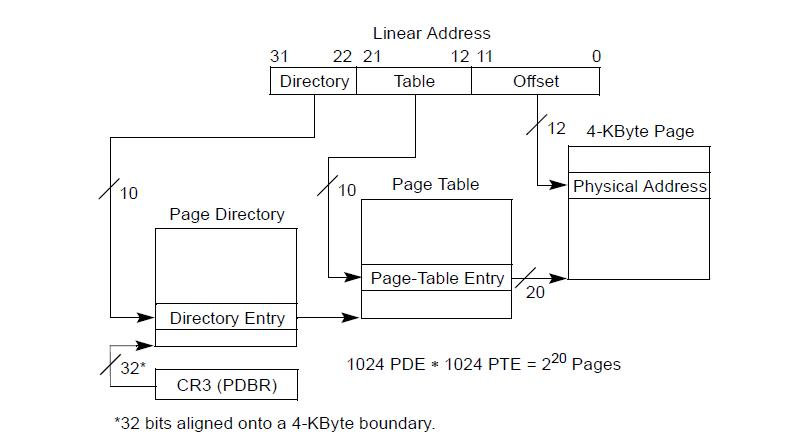
\includegraphics[scale=0.5]{lab2.pt.jpg}

可以看到JOS采用了两级页表。给定一个32位线性地址,它可以被拆分为10+10+12位:高10位是该线性地址在页目
\lstinline|pgdir|中对应的页目录项PDE的下标,从而得到页目录项PDE。页目录项PDE也是一个 32
位无符号整数,其中高20位保存的是地址,低12位使用相关的信息;中10位是该线性地址在页表中对应页表项PTE的下标,从而得到页表项PTE,
页表项PTE和页目录项PDE的结构相同;低12位则是数据在物理页内的偏移。
对于页目录项和页目录项,除了高20位表示地址外,其余的低12位在\lstinline|mmu.h|中有如下定义:
\begin{lstlisting}[title=inc/mmu.h]
#define PTE_P		0x001	// Present
#define PTE_W		0x002	// Writeable
#define PTE_U		0x004	// User
#define PTE_PWT		0x008	// Write-Through
#define PTE_PCD		0x010	// Cache-Disable
#define PTE_A		0x020	// Accessed
#define PTE_D		0x040	// Dirty
#define PTE_PS		0x080	// Page Size
#define PTE_G		0x100	// Global
\end{lstlisting}
其中常用的\lstinline|PTE_P|表示页存在,\lstinline|PTE_W|表示可以写,\lstinline|PTE_U|表示用户有权限访问,\lstinline|PTE_PS|表示这是一个4M的页。

x86还提供了TLB机制。这是为了提高地址转换的效率,系统将最常用到的页表数据保存在TLB,如果TLB命中时,则跳过页式转换。因此,每次更改页目录和页表时,都要刷新TLB。JOS中,在我们采用的是利用\lstinline|MOV|指令重写\lstinline|%cr3|,具体操作为\lstinline|tlb_invalidate()|。

\begin{framed}
\noindent\textbf{Exercise 3} While GDB can only access QEMU's memory by virtual address, it's often useful to be able to inspect physical memory while setting up virtual memory. Review the QEMU monitor commands from the lab tools guide, especially the \lstinline|xp| command, which lets you inspect physical memory. To access the QEMU monitor, press \lstinline|Ctrl-a c| in the terminal (the same binding returns to the serial console).

Use the xp command in the QEMU monitor and the \lstinline|x| command in GDB to inspect memory at corresponding physical and virtual addresses and make sure you see the same data.

Our patched version of QEMU provides an \lstinline|info pg| command that may also prove useful: it shows a compact but detailed representation of the current page tables, including all mapped memory ranges, permissions, and flags. Stock QEMU also provides an \lstinline|info mem| command that shows an overview of which ranges of virtual memory are mapped and with what permissions. 
\end{framed}
在这个练习中,我们可以通过在QEMU中断来查看操作系统的信息。一些有用的操作如下:

\begin{center}
\begin{tabular}{rl}
x/Nx addr & 查看addr开始的虚拟地址 \\
xp/Nx addr & 查看addr开始的物理地址 \\
info mem & 显示虚拟地址映射到的物理地址以及权限 \\
info pg & 显示页目录,页表结构
\end{tabular}
\end{center}

\begin{framed}
\textbf{Question}
1. Assuming that the following JOS kernel code is correct, what type should variable \lstinline|x| have, \lstinline|uintptr_t| or \lstinline|physaddr_t|?
\begin{lstlisting}[frame=none,aboveskip=-1.5em]
    	mystery_t x;
    	char* value = return_a_pointer();
    	*value = 10;
    	x = (mystery_t) value;
\end{lstlisting}
\end{framed}
\lstinline|x|保存的是value对应的虚拟地址,所以\lstinline|x|的类型是\lstinline|uintptr_t|。

\begin{framed}
\noindent\textbf{Exercise 4}In the file \lstinline|kern/pmap.c|, you must implement code for the following functions.
\begin{lstlisting}[frame=none,aboveskip=-1.5em]
pgdir_walk()
boot_map_region()
page_lookup()
page_remove()
page_insert()
\end{lstlisting}
\lstinline|check_page()|, called from \lstinline|mem_init()|, tests your page table management routines. You should make sure it reports success before proceeding.
\end{framed}

\subsection{\lstinline|pgdir_walk()|}
这个函数的实现要求是,给定页目录指针\lstinline|pgdir|,需要返回一个对应于线性地址\lstinline|va|的页表项指针。
需要注意一下几点:
\begin{packed_enum}
\item 相关页表项可能不存在。
\item 这时如果\lstinline|create == false|,那么返回\lstinline|NULL|;否则,创建新的页表项所对应的页。
\item 如果创建失败,返回\lstinline|NULL|,否则清空页,增加物理页引用计数,设置页表项内容,返回该页指针。
\end{packed_enum}

\begin{lstlisting}[title=kern/pmap.c,numbers=left]
pte_t *
pgdir_walk(pde_t *pgdir, const void *va, int create)
{
	pgdir = &pgdir[PDX(va)];
	struct PageInfo* info;
	if (*pgdir & PTE_PS)
		return pgdir;
	if (*pgdir & PTE_P) {
		return (pte_t*)KADDR(PTE_ADDR(*pgdir)) + PTX(va);
	} else {
		if (create == false)
			return NULL;
		else {
			info = page_alloc(ALLOC_ZERO);
			if (info == NULL)
				return NULL;
			else {
				info->pp_ref++;
				*pgdir = page2pa(info) | PTE_P | PTE_W | PTE_U;
				return (pte_t*)KADDR(PTE_ADDR(*pgdir)) + PTX(va);
			}
		}
	}
}
\end{lstlisting}

第4行首先计算页目录项。

第6、7行用于判断是否是4MB的页,如果是就直接返回页目录,因为4MB的页不需要二级存储。

第9行适用于页表项存在的情况。注意先要使用\lstinline|KADDR(PTE_ADDR(*pgdir))|,获取对应的页目录表基地值,再加上\lstinline|PTX(va)|作为页目录表的偏移。

第12行代表\lstinline|create==false|的情况,直接返回空。

第16行代表内存溢出的情况,也返回空。

第18到20行代表新建页表项的页,并且更新页表项内容,也就是设置高20位为新建页的物理地址,并且设置存在,可写,用户可访问的标志位,返回值与第9行相同。

写代码的时候一定要思路清晰,哪里用物理地址,哪里用虚拟地址;简单地来说,放在页目录项和页表项中的都是物理地址,程序代码中的基本全是虚拟地址。

\subsection{\lstinline|boot_map_region()|}

这个函数的实现要求如下,将\lstinline|pgdir|表中虚拟地址[\lstinline|[va, va+size)|]映射到[\lstinline|[pa, pa+size)|。注意需要按照\lstinline|PGSIZE|对齐。并且这个函数只是改变静态的映射,不改变任何结构,因此\lstinline|pp_ref|不需要更改。

实现如下:
\begin{lstlisting}[title=kern/pmap.c]
static void
boot_map_region(pde_t *pgdir, uintptr_t va, size_t size, physaddr_t pa, int perm)
{
	// Fill this function in
	pte_t *pgtable;
	size_t i, c = PGNUM(size);
	size_t step = (perm & PTE_PS) ? NPDENTRIES : 1;
	for (i = 0; i < c; i+= step) {
		pgtable = (perm & PTE_PS) ? &pgdir[PDX(va)] : pgdir_walk(pgdir, (const void*)va, true);
		if (pgtable == NULL)
			panic("boot_map_region(): out of memory");
		*pgtable = pa | perm | PTE_P;
		va += PGSIZE * step;
		pa += PGSIZE * step;
	}
}
\end{lstlisting}
我们只需要通过\lstinline|pgdir_walk|获取页目录项地址,然后更改相应页目录项就可以了。这里也是Challenge 1涉及的函数之一,需要考虑到4M页的情况。

\subsection{\lstinline|page_lookup()|}
这个函数需要根据指定页目录\lstinline|pgdir|和虚拟地址\lstinline|va|,如果物理页存在,那么返回物理页信息\lstinline|PageInfo*|;否则返回 NULL。如果还指定了\lstinline|pte_store|,则还需要把它设成相应的页表项地址。实现如下:

\begin{lstlisting}[title=kern/pmap.c]
struct PageInfo *
page_lookup(pde_t *pgdir, void *va, pte_t **pte_store)
{
	pte_t *pgtable = pgdir_walk(pgdir, va, false);
	if (pte_store)
		*pte_store = pgtable;
	if (pgtable == NULL)
		return NULL;
	if (*pgtable & PTE_P)
		return pa2page(PTE_ADDR(*pgtable));
	return NULL;
}
\end{lstlisting}

可以看到,其实\lstinline|page_lookup|就是\lstinline|pgdir_walk|的一个包装,当然它不会创建新页。

\subsection{\lstinline|page_remove()|}
这个函数根据指定页目录\lstinline|pgdir|和虚拟地址\lstinline|va|,如果\lstinline|va|有映射,那么移除;否则返回。
此外,要将物理页的引用计数减一,如果物理页引用计数减到零,要将物理页放回空闲页链表中。同时还要将页表项清零。

由于在调用\lstinline|page_decref|时,会自动判断引用计数是否为零,所以直接调用就可以了。实现如下:
\begin{lstlisting}
void
page_remove(pde_t *pgdir, void *va)
{
	pte_t *pgtable;
	struct PageInfo *info = page_lookup(pgdir, va, &pgtable);
	if (info == NULL)
		return;
	*pgtable = 0;
	tlb_invalidate(pgdir, va);
	page_decref(info);
}
\end{lstlisting}

\subsection{\lstinline|page_insert()|}
此函数的主要功能如下:根据页目录\lstinline|pgdir|和虚拟地址\lstinline|va|映射到物理页信息指针\lstinline|pp|对应的物理地址,同时设置权限位为\lstinline!perm|PTE_P!。
\begin{packed_enum}
\item 如果\lstinline|va|已经映射到某个物理地址,应先将该物理地址所在物理页\lstinline|page_remove()|。
\item 如果需要的话,可以新建并分配一个页目录。
\item 插入成功的话,\lstinline|pp_ref|自增。
\item 使TLB失效。
\end{packed_enum}
\lstinline|page_insert|这个名字有一些误导,其实应该表示成添加映射之类的词语,比如\lstinline|page_map()|。另外,注释中还提到了如果原来物理地址与将要分配的地址相同这样一种情况,但是注释中又不鼓励我们显式地区分这样的情况。最后实在是没有办法,还是显式地区分了一下:
\begin{lstlisting}[title=kern/pmap.c]
int
page_insert(pde_t *pgdir, struct PageInfo *pp, void *va, int perm)
{
	// Fill this function in
	pte_t *pgtable = pgdir_walk(pgdir, va, true);
	if (pgtable == NULL)
		return -E_NO_MEM;
	if (*pgtable & PTE_P) {
		if (PTE_ADDR(*pgtable) == page2pa(pp))
			pp->pp_ref--;
		else
			page_remove(pgdir, va);
	}
	pp->pp_ref++;
	*pgtable = page2pa(pp) | perm | PTE_P;
	return 0;
}
\end{lstlisting}
其中用到的一个小技巧是,在原来物理地址与将要分配的地址相同的情况下,先将\lstinline|pp->pp_ref--|,再将\lstinline|pp->pp_ref++|。虽然看起来没有什么必要,但这有可能就是注释的意思。另外还有一点是,由于在\lstinline|page_remove|的时候,已经调用过\lstinline|tlb_invalidate|了,所以不需要在该函数中调用了。

\section{Kernel Address Space}
\begin{framed}
\textbf{Exercise 5} Fill in the missing code in \lstinline|mem_init()| after the call to \lstinline|check_page()|.

Your code should now pass the \lstinline|check_kern_pgdir()| and \lstinline|check_page_installed_pgdir()| checks. 
\end{framed}
这一部分有三个步骤,首先要将线性地址\lstinline|UPAGES|映射到\lstinline|pages|数组。
要求:
\begin{packed_enum}
\item 对于新的在\lstinline|UPAGES|的页面,权限为\lstinline!PTE_U | PTE_P!。
\item 对于在\lstinline|pages|的页面,权限为\lstinline!PTE_W | PTE_P!
\end{packed_enum}
这里我们使用\lstinline|boot_map_region|来进行映射,
\begin{lstlisting}
boot_map_region(kern_pgdir, 
	UPAGES, 
	ROUNDUP(npages * sizeof(struct PageInfo), PGSIZE), 
	PADDR(pages), 
	PTE_U | PTE_P);
boot_map_region(kern_pgdir,
	(uintptr_t)pages,
	ROUNDUP(npages * sizeof(struct PageInfo), PGSIZE),
	PADDR(pages),
	PTE_W | PTE_P
	);
\end{lstlisting}

然后将虚拟地址[\lstinline|KSTACKTOP-KSTKSIZE, KSTACKTOP|)映射到由\lstinline|bootstack|指定的物理地址。注意这里的\lstinline|bootstack|是虚拟地址。这里的实现倒不难,实现如下:
\begin{lstlisting}
boot_map_region(kern_pgdir,
	KSTACKTOP-KSTKSIZE,
	KSTKSIZE,
	PADDR(bootstack),
	PTE_W | PTE_P);
\end{lstlisting}
对于[\lstinline|KSTACKTOP-PTSIZE, KSTACKTOP-KSTKSIZE|),这些虚拟地址空间中是栈的缓冲区,提升了JOS系统的稳健性。

最后从KERNBASE开始映射到整个物理内存空间,这样在页式转换打开以后,Kernel也能使用统一的虚拟地址来访问内存数据。实现如下:
\begin{lstlisting}
boot_map_region(kern_pgdir,
	KERNBASE,
	~KERNBASE,
	0,
	PTE_W | PTE_P);
\end{lstlisting}

在完成了\lstinline|mem_init|以后,Lab2的主要实验就完成了。

\begin{center}
\includegraphics[scale=0.4]{lab2.result.png}
\end{center}

\begin{framed}
\textbf{Question}

2. What entries (rows) in the page directory have been filled in at this point? What addresses do they map and where do they point? In other words, fill out this table as much as possible:

\begin{tabular}{lll}
Entry & Base Virtual Address & Points to (logically)\\
1023	  & ?	& Page table for top 4MB of phys memory\\
1022	  & ?	& ?\\
.	  & ?	& ?\\
.	  & ?	& ?\\
.	  & ?	& ?\\
2	  & 0x00800000	& ?\\
1	  & 0x00400000	& ?\\
0	  & 0x00000000	& [see next question]\\
\end{tabular}

3. (From Lecture 3) We have placed the kernel and user environment in the same address space. Why will user programs not be able to read or write the kernel's memory? What specific mechanisms protect the kernel memory?

4. What is the maximum amount of physical memory that this operating system can support? Why?

5. How much space overhead is there for managing memory, if we actually had the maximum amount of physical memory? How is this overhead broken down?

6. Revisit the page table setup in kern/entry.S and kern/entrypgdir.c. Immediately after we turn on paging, EIP is still a low number (a little over 1MB). At what point do we transition to running at an EIP above KERNBASE? What makes it possible for us to continue executing at a low EIP between when we enable paging and when we begin running at an EIP above KERNBASE? Why is this transition necessary? 
\end{framed}

\noindent\textbf{Question 2}
其实只需要在QEMU中按下Ctrl-a再按c,进入QEMU输入info pg即可获得页目录信息就可以了。输出结果如下:
\begin{lstlisting}[aboveskip=-1.5em]
(qemu) info pg
VPN range     Entry         Flags        Physical page
[ef000-ef3ff]  PDE[3bc]     -------UWP
  [ef000-ef020]  PTE[000-020] -------U-P 0011a-0013a
[ef400-ef7ff]  PDE[3bd]     -------U-P
  [ef7bc-ef7bc]  PTE[3bc]     -------UWP 003fd
  [ef7bd-ef7bd]  PTE[3bd]     -------U-P 00119
  [ef7bf-ef7bf]  PTE[3bf]     -------UWP 003fe
  [ef7c0-ef7d0]  PTE[3c0-3d0] ----A--UWP 003ff 003fc 003fb 003fa 003f9 003f8 ..
  [ef7d1-ef7ff]  PTE[3d1-3ff] -------UWP 003ec 003eb 003ea 003e9 003e8 003e7 ..
[efc00-effff]  PDE[3bf]     -------UWP
  [efff8-effff]  PTE[3f8-3ff] --------WP 0010e-00115
[f0000-f03ff]  PDE[3c0]     ----A--UWP
  [f0000-f0000]  PTE[000]     --------WP 00000
  [f0001-f009f]  PTE[001-09f] ---DA---WP 00001-0009f
  [f00a0-f00b7]  PTE[0a0-0b7] --------WP 000a0-000b7
  [f00b8-f00b8]  PTE[0b8]     ---DA---WP 000b8
  [f00b9-f00ff]  PTE[0b9-0ff] --------WP 000b9-000ff
  [f0100-f0105]  PTE[100-105] ----A---WP 00100-00105
  [f0106-f0114]  PTE[106-114] --------WP 00106-00114
  [f0115-f0115]  PTE[115]     ---DA---WP 00115
  [f0116-f0117]  PTE[116-117] --------WP 00116-00117
  [f0118-f0119]  PTE[118-119] ---DA---WP 00118-00119
  [f011a-f011a]  PTE[11a]     ----A---WP 0011a
  [f011b-f011b]  PTE[11b]     ---DA---WP 0011b
  [f011c-f013a]  PTE[11c-13a] ----A---WP 0011c-0013a
  [f013b-f03bd]  PTE[13b-3bd] ---DA---WP 0013b-003bd
  [f03be-f03ff]  PTE[3be-3ff] --------WP 003be-003ff
[f0400-f3fff]  PDE[3c1-3cf] ----A--UWP
  [f0400-f3fff]  PTE[000-3ff] ---DA---WP 00400-03fff
[f4000-f43ff]  PDE[3d0]     ----A--UWP
  [f4000-f40fe]  PTE[000-0fe] ---DA---WP 04000-040fe
  [f40ff-f43ff]  PTE[0ff-3ff] --------WP 040ff-043ff
[f4400-fffff]  PDE[3d1-3ff] -------UWP
  [f4400-fffff]  PTE[000-3ff] --------WP 04400-0ffff
\end{lstlisting}
我们只需要关注包含PDE行,就可以在第一个中括号内找到PDE对应的逻辑地址,第二个中括号内找到PDE的下标。

\noindent\textbf{Question 3}
如果用户可以读写Kernel内存的话,用户程序的bug可能会覆盖Kernel的数据,导致系统崩溃或者部分功能失效。用户程序也可能读取一些关键的Kernel信息以及其他进程的信息。

Kernel需要防止用户程序访问[\lstinline|ULIM,KERNBASE|)的虚拟地址空间,以防止用户读取或改写Kernel数据。在x86中的页目录项PDE和页表项PTE均有权限设置,如U/S, R/W,这使得用户程序无法访问到这些地址对应的实际内存,也就无法读取或者写入被保护的地址。

\noindent\textbf{Question 4}
最大物理内存理应是4GB,但是由于\lstinline|UPAGES|到\lstinline|UVPT|有分配的固定大小PTSIZE,所以由\lstinline|PTSIZE / SIZEOF(PAGEINFO) * PGSIZE = 2GB|知最大物理内存是2GB。

\noindent\textbf{Question 5}
本来一个页目录对应1个物理页,页表对应了1024张物理页,但是由于页目录将自身当成了一个页表,所以总开销就是1024个物理页也就是4MB。所以这也就组成了这些额外开销的全部。

\begin{lstlisting}[title=kern/pmap.c]
    // Recursively insert PD in itself as a page table, to form
    // a virtual page table at virtual address UVPT.
    kern_pgdir[PDX(UVPT)] = PADDR(kern_pgdir) | PTE_U | PTE_P;
\end{lstlisting}

\noindent\textbf{Question 6}

\begin{lstlisting}[title=kern/entry.S,numbers=left,firstnumber=64]
	# Now paging is enabled, but we're still running at a low EIP
	# (why is this okay?).  Jump up above KERNBASE before entering
	# C code.
	mov	$relocated, %eax
	jmp	*%eax
\end{lstlisting}
第68行使得\lstinline|%eip|超过了\lstinline|KERNBASE|。
\lstinline|%eip|能够在低地址段执行是因为在\lstinline|entrypgdir.c|中有一个临时的页表,将虚拟地址[\lstinline|0, 4MB|)和[\lstinline|KERNBASE, KERNBASE+4MB|)都映射到[\lstinline|0, 4MB|)。

\begin{lstlisting}[title=kern/entrypgdir.c,numbers=left,firstnumber=6]
// The entry.S page directory maps the first 4MB of physical memory
// starting at virtual address KERNBASE (that is, it maps virtual
// addresses [KERNBASE, KERNBASE+4MB) to physical addresses [0, 4MB)).
// We choose 4MB because that's how much we can map with one page
// table and it's enough to get us through early boot.  We also map
// virtual addresses [0, 4MB) to physical addresses [0, 4MB); this
// region is critical for a few instructions in entry.S and then we
// never use it again.
//
// Page directories (and page tables), must start on a page boundary,
// hence the "__aligned__" attribute.  Also, because of restrictions
// related to linking and static initializers, we use "x + PTE_P"
// here, rather than the more standard "x | PTE_P".  Everywhere else
// you should use "|" to combine flags.
__attribute__((__aligned__(PGSIZE)))
pde_t entry_pgdir[NPDENTRIES] = {
	// Map VA's [0, 4MB) to PA's [0, 4MB)
	[0]
		= ((uintptr_t)entry_pgtable - KERNBASE) + PTE_P,
	// Map VA's [KERNBASE, KERNBASE+4MB) to PA's [0, 4MB)
	[KERNBASE>>PDXSHIFT]
		= ((uintptr_t)entry_pgtable - KERNBASE) + PTE_P + PTE_W
};
\end{lstlisting}
\section{Challenges}
我完成了Challenge 1和Challenge 2。
\subsection{Challenge 1}
\begin{framed}
We consumed many physical pages to hold the page tables for the \lstinline|KERNBASE| mapping. Do a more space-efficient job using the \lstinline|PTE_PS| ("Page Size") bit in the page directory entries. This bit was not supported in the original 80386, but is supported on more recent x86 processors. You will therefore have to refer to Volume 3 of the current Intel manuals. Make sure you design the kernel to use this optimization only on processors that support it!
\end{framed}
本Challenge需要缩减将\lstinline|KERNBASE|开始的虚拟地址映射到整块物理内存的开销。可以通过在页目录项PDE中打开\lstinline|PTE_PS|位,从而开启4M页机制,节省页表,提高命中率。另外需要检测处理器是否支持这一个选项。4M页机制开启时如下图所示:

\begin{center}
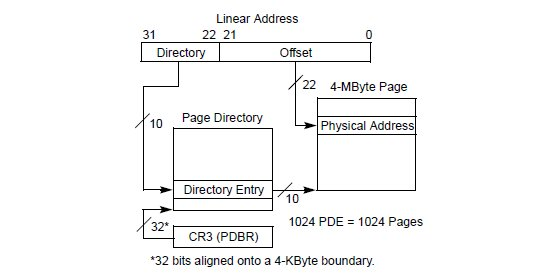
\includegraphics[scale=0.5]{lab2.pe.png}
\end{center}

从图上我们看出,线性地址被划分为10+22位:高10位是对应页目录项PDE在页目录\lstinline|pgdir|中的下标,PDE中也有中我们立即得到物理页的起始地址(实际指定上只有高 10 位有效);低22位是物理页内的偏移。

我们的代码修改如下:

\begin{lstlisting}[title=mem\_init()]
    ...
	boot_map_region(kern_pgdir,
		KERNBASE,
		~KERNBASE,
		0,
		PTE_W | PTE_P | PTE_PS);

	cr4 = rcr4();
	cr4 |= CR4_PSE;
	lcr4(cr4);

	lcr3(PADDR(kern_pgdir));
	...
\end{lstlisting}
这里需要注意的是,在修改\lstinline|%cr3|前需要设置\lstinline|%cr4|的\lstinline|CR4_PSE|,从而开启扩展。

\begin{lstlisting}[title=boot\_map\_region()]
static void
boot_map_region(pde_t *pgdir, uintptr_t va, size_t size, physaddr_t pa, int perm)
{
	// Fill this function in
	pte_t *pgtable;
	size_t i, c = PGNUM(size);
	size_t step = (perm & PTE_PS) ? NPDENTRIES : 1;
	for (i = 0; i < c; i+= step) {
		pgtable = (perm & PTE_PS) ? &pgdir[PDX(va)] : pgdir_walk(pgdir, (const void*)va, true);
		if (pgtable == NULL)
			panic("boot_map_region(): out of memory");
		*pgtable = pa | perm | PTE_P;
		va += PGSIZE * step;
		pa += PGSIZE * step;
	}
}
\end{lstlisting}
这里判断是否设置\lstinline|PTE_PS|变量,如果设置了,那么每一次\lstinline|va|和\lstinline|pa|的步长都会乘以\lstinline|NPDENTRIES=1024|。

\begin{lstlisting}[title=pgdir\_walk()]
pte_t *
pgdir_walk(pde_t *pgdir, const void *va, int create)
{
	pgdir = &pgdir[PDX(va)];
	struct PageInfo* info;
	if (*pgdir & PTE_PS)
		return pgdir;
    ...
}
\end{lstlisting}
如果当前页目录项设置了\lstinline|PTE_PS|位,那么直接返回页目录项。

完成了上述修改以后我们的Challenge基本完成,但注意,相关的测试函数还没有修改!

\begin{lstlisting}[title=check\_kern\_pgdir()]
	// check phys mem
	for (i = 0; i < npages * PGSIZE; i += PGSIZE * NPDENTRIES)
		assert(check_va2pa(pgdir, KERNBASE + i) == i);
\end{lstlisting}
这里需要对\lstinline|i|的步长进行修改!否则会抛出Triple fault(这个错误在调试的时候真是太常见了)。

\begin{lstlisting}[title=check\_va2pa()]
static physaddr_t
check_va2pa(pde_t *pgdir, uintptr_t va)
{
	pte_t *p;

	pgdir = &pgdir[PDX(va)];
	if (!(*pgdir & PTE_P))
		return ~0;
	if (*pgdir & PTE_PS)
		return PTE_ADDR(*pgdir);
	p = (pte_t*) KADDR(PTE_ADDR(*pgdir));
	if (!(p[PTX(va)] & PTE_P))
		return ~0;
	return PTE_ADDR(p[PTX(va)]);
}
\end{lstlisting}
如果检查的页目录项设置了\lstinline|PTE_PS|位,那么直接返回页目录项。

到此位置,我们完成了Challenge 1,结果如下(可以看到结果相比Question 2)缩短了很多。

\begin{center}
\includegraphics[scale=0.4]{lab2.c1.png}
\end{center}

至于处理器是否支持4M分页,在网上搜索了一下,貌似x86架构都支持4M分页,无论是x86还是x86\_64。尽管我的ubuntu是64位的,运行起来也没有任何问题。所以即使我们找到了检测是否支持4M分页的方法,也很难找到不支持的机器来测试。

\subsection{Challenge 2}
\begin{framed}
Extend the JOS kernel monitor with commands to:

1. Display in a useful and easy-to-read format all of the physical page mappings (or lack thereof) that apply to a particular range of virtual/linear addresses in the currently active address space. For example, you might enter 'showmappings 0x3000 0x5000' to display the physical page mappings and corresponding permission bits that apply to the pages at virtual addresses 0x3000, 0x4000, and 0x5000.

2. Explicitly set, clear, or change the permissions of any mapping in the current address space.

3. Dump the contents of a range of memory given either a virtual or physical address range. Be sure the dump code behaves correctly when the range extends across page boundaries!

Do anything else that you think might be useful later for debugging the kernel. (There's a good chance it will be!)

\end{framed}
Challenge 2的实现都比较简单,前两项可以直接使用\lstinline|pgdir_walk|来获取页表项进行操作。最后一项可以利用\lstinline|KADDR|宏来实现,这里直接贴上代码。

\begin{lstlisting}[title=monitor.c]
...

#include <kern/pmap.h>

...
static struct Command commands[] = {
	{ "help", "Display this list of commands", mon_help },
	{ "kerninfo", "Display information about the kernel", mon_kerninfo },
	{ "backtrace", "Display stack", mon_backtrace },
	{ "map", "Display mapping", mon_map },
	{ "set", "Set mapping", mon_set },
	{ "xp", "Dump physical memory", mon_xp },
	{ "xv", "Dump virtual memory", mon_xv },
};

...

int
mon_map(int argc, char **argv, struct Trapframe *tf)
{
	size_t start;
	size_t end;
	size_t i;
	char status[10];
	start = strtol(argv[1], NULL, 0);
	end = strtol(argv[2], NULL, 0);
	pte_t* pgtable;
	if (start < 0 || start > end) {
		cprintf("Invalid parameters[start=%08x, end=%08x]\n", start, end);
		return 0;
	}
	strcpy(status, "---------");
	start = ROUNDDOWN(start, PGSIZE);
	for (i = start; i < end; i += PGSIZE) {
		pgtable = pgdir_walk(kern_pgdir, (const void*)i, true);
		status[0] = (*pgtable & PTE_G)   ? 'G' : '-';
		status[1] = (*pgtable & PTE_PS)  ? 'S' : '-';
		status[2] = (*pgtable & PTE_D)   ? 'D' : '-';
		status[3] = (*pgtable & PTE_A)   ? 'A' : '-';
		status[4] = (*pgtable & PTE_PCD) ? 'C' : '-';
		status[5] = (*pgtable & PTE_PWT) ? 'T' : '-';
		status[6] = (*pgtable & PTE_U)   ? 'U' : '-';
		status[7] = (*pgtable & PTE_W)   ? 'W' : '-';
		status[8] = (*pgtable & PTE_P)   ? 'P' : '-';
		cprintf("[%5x-%5x] %s %5x\n", PGNUM(i), PGNUM(i)+1, status, PGNUM(*pgtable));
	}
	return 0;
}

int
mon_set(int argc, char **argv, struct Trapframe *tf)
{
	size_t page;
	size_t flag;
	char status[10];
	pte_t* pgtable;
	page = strtol(argv[1], NULL, 0);
	flag = strtol(argv[2], NULL, 0);
	if (page < 0 || page > KERNBASE) {
		cprintf("Invalid parameters[page=%08x]\n", page);
		return 0;
	}
	strcpy(status, "---------");
	page = ROUNDDOWN(page, PGSIZE);
	pgtable = pgdir_walk(kern_pgdir, (const void*)page, true);
	*pgtable = PTE_ADDR(*pgtable) | flag;
	status[0] = (*pgtable & PTE_G)   ? 'G' : '-';
	status[1] = (*pgtable & PTE_PS)  ? 'S' : '-';
	status[2] = (*pgtable & PTE_D)   ? 'D' : '-';
	status[3] = (*pgtable & PTE_A)   ? 'A' : '-';
	status[4] = (*pgtable & PTE_PCD) ? 'C' : '-';
	status[5] = (*pgtable & PTE_PWT) ? 'T' : '-';
	status[6] = (*pgtable & PTE_U)   ? 'U' : '-';
	status[7] = (*pgtable & PTE_W)   ? 'W' : '-';
	status[8] = (*pgtable & PTE_P)   ? 'P' : '-';
	cprintf("[%5x-%5x] %s %5x\n", PGNUM(page), PGNUM(page)+1, status, PGNUM(*pgtable));
	return 0;
}

int
mon_xp(int argc, char **argv, struct Trapframe *tf)
{
	size_t start;
	size_t length;
	size_t i;
	start = strtol(argv[1], NULL, 0);
	length = strtol(argv[2], NULL, 0);
	for (i = 0; i < length; i+=4, start+=4) {
		cprintf("[%08x]: 0x%08x 0x%08x 0x%08x 0x%08x\n", 
			start, 
			*((uint32_t*)KADDR(start)),
			*((uint32_t*)KADDR(start+4)),
			*((uint32_t*)KADDR(start+8)),
			*((uint32_t*)KADDR(start+12))
		);
	}
	return 0;
}

int
mon_xv(int argc, char **argv, struct Trapframe *tf)
{
	size_t start;
	size_t length;
	size_t i;
	start = strtol(argv[1], NULL, 0);
	length = strtol(argv[2], NULL, 0);
	for (i = 0; i < length; i+=4, start+=4) {
		cprintf("[%08x]: 0x%08x 0x%08x 0x%08x 0x%08x\n", 
			start, 
			*((uint32_t*)(start)),
			*((uint32_t*)(start+4)),
			*((uint32_t*)(start+8)),
			*((uint32_t*)(start+12))
		);
	}
	return 0;
}
\end{lstlisting}

实验结果如下,可以看到前两项组合后成功,最后一项也于QEMU的dump值相等。

\begin{center}
\includegraphics[scale=0.4]{lab2.c2.png}
\end{center}

\subsection{Challenge 4}
\begin{framed}
Since our JOS kernel's memory management system only allocates and frees memory on page granularity, we do not have anything comparable to a general-purpose \lstinline|malloc/free| facility that we can use within the kernel. This could be a problem if we want to support certain types of I/O devices that require physically contiguous buffers larger than 4KB in size, or if we want user-level environments, and not just the kernel, to be able to allocate and map 4MB superpages for maximum processor efficiency. (See the earlier challenge problem about \lstinline|PTE_PS|.)

Generalize the kernel's memory allocation system to support pages of a variety of power-of-two allocation unit sizes from 4KB up to some reasonable maximum of your choice. Be sure you have some way to divide larger allocation units into smaller ones on demand, and to coalesce multiple small allocation units back into larger units when possible. Think about the issues that might arise in such a system. 
\end{framed}

这个Challenge希望让Kernel能够支持从4KB开始到4MB(假设)任意2的幂Byte的大小的页面。当然这里指的是连续的物理页。这个实现就是伙伴系统。如果没有合适大小的页框,我们必须要对更大的页框进行分割;如果页框被释放,那么要还要对可能的页框进行合并。JOS利用\lstinline|page_free_list|来管理4KB的页,但为了实现这个Challenge的内容,我们需要把所有的可用页框分为11组,用11个链表管理,每个链表链接的可用页框大小为 4KB,8 KB,16 KB,32 KB,64 KB,128 KB,256 KB,512 KB,1MB,2MB,4MB;而且需要让每个页框的起始物理地址对齐。
假设现在我们要申请一个128KB的连续物理地址,我们首先从128KB页框链表查找可用页框,如果有就返回;否则就递归地从256KB页框链表中找一个可用的,将它分成2个128KB 的页框,一个用于返回,一个加入128KB的链表。释放页框的时候,需要检查前后相邻的是否也是可用,如果可用就合并,加入上一级的可用页框列表。
这个Challenge暂时没有实现。

\section{Tips}
\begin{packed_enum}
\item 一定要记得什么时候用虚拟地址,什么时候用物理地址。
\item 调试时用类似\lstinline|warn("%d", i)|的语句来测试断点或者输出相关值!
\item 碰到Triple Fault一定要耐心调试!
\end{packed_enum}

\section{References}
北京大学操作系统实习(实验班)报告, 黄睿哲.

操作系统JOS实习第二次报告, 张弛


\end{document}